\documentclass[12pt]{scrartcl}

%\input{../Packages.tex}
%\input{../FormatAndHeader.tex}

\input{../Style Template/Packages.tex}
\input{../Style Template/FormatAndHeader.tex}

\setcounter{sheetnr}{1}
\setcounter{enumi}{2}

\begin{document}

\exercise{}
    \begin{itemize}
        \item[\theenumi.1)]
            Utility beschreibt, ob ein Produkt seine Funktion erfolgreich erfüllt.
            Usability gibt an, inwieweit der Nutzer von dem Produkt bei der Benutzung unterstützt wird.
            Likability beschreibt nur, ob ein Produkt gemocht wird, unabhängig von seiner Effizienz und Nutzerfreundlichkeit.
        \item[\theenumi.2)]Lernbarkeit, Effizienz, Einprägsamkeit, Fehlerrate, Befriedigung 
    \end{itemize}

\setcounter{enumi}{4}
\exercise{}
\begin{itemize}
    \item[\theenumi.1)] Die unabhängige Variable ist der Diagrammtyp und die abhängige Variable ist die Ablesezeit.
    \item[\theenumi.2)] Die unabhängige Variable ist die Anzahl der Punkte in der Übung und die abhängige Variable ist die Note in der Klausur.
\end{itemize}

\stepcounter{enumi}
\exercise{}

\begin{itemize}
    \item[\theenumi.1)] Latin square design: Es ist in dieser Studie sinnvoll, da durch die verschiedenen Reihenfolgen der Diagramme 
                        ausgeschlossen werden kann, dass die Ergebnisse von der gewählten Reihenfolge abhängt. Zudem kann die Anzahl der Teilnehmer geringer als bei einer within-Gruppenstudie gehalten werden, 
                        da nur 3 Sequenzen anstatt 6 Sequenzen durchlaufen und vorbereitet werden müssen.
	\item[\theenumi.2)] Unabhängige Variablen sind die Anzahl der Datenwerte (7,12,24) und die Art des Diagramms
	Unabhängige Variablen ist die Zeit
	\item[\theenumi.3)] Die Rückmeldung direkt nach der Eingabe kann ein Problem sein, weil dadurch die Teilnehmer entweder demotivierter oder selbstbewusster bzw. leichtsinniger bei der Antwortgabe werden.
	Ein mögliches Problem könnte sein, dass nur Probanden betrachtet wurden die einen hohen akademischen Abschluss haben. Sie sind dadurch schon vertrauter mit Diagrammen aller Art.
\end{itemize}


\stepcounter{enumi}
\exercise{}
\begin{itemize}
    \item[\theenumi.1)] \, \\
        \begin{tabular}{c c c}
            \textbf{Tag} & \textbf{Julia} & \textbf{Salome}\\ \hline
            Mittwoch & 390 Min & 600 Min\\ \hline
            Donnerstag & 720 Min & 630 Min\\ \hline
            Freitag & 0 Min & 390 Min\\ \hline
            Samstag & 0 Min & 30 Min\\ \hline
            Sonntag & 0 Min & 330 Min\\ \hline
        \end{tabular}
    \item[\theenumi.2)] Durchschnitt Julia: 222 Min\\
                        Durchschnitt Salome: 396 Min
    \item[\theenumi.3)] \, \\
        \begin{tabular}{c | c c}
            & \textbf{Julia} & \textbf{Salome}\\ \hline
            \textbf{Durchschnitt} & 222 Min& 396 Min\\\hline
            \textbf{Standardabweichung} & 291.232 Min & 277.013 Min \\\hline
            \textbf{Median} & 0 Min & 390 Min
        \end{tabular}
    \item[\theenumi.4)] \, \\

    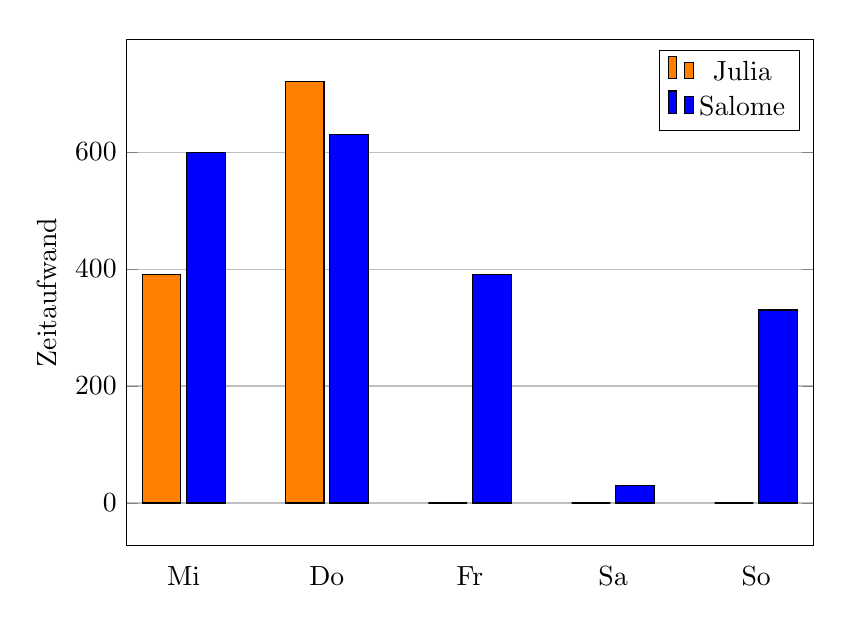
\begin{tikzpicture}
    \begin{axis}[
        width  = 0.85*\textwidth,
        height = 8cm,
        major x tick style = transparent,
        ybar,
        bar width=14pt,
        ymajorgrids = true,
        ylabel = {Zeitaufwand},
        symbolic x coords={Mi, Do, Fr, Sa, So},
        xtick = data,
        scaled y ticks = false,
    ]
      \addplot [ybar, fill = orange] coordinates {(Mi, 390)(Do, 720) (Fr, 0) (Sa, 0) (So, 0)};
      \addplot [ybar, fill = blue] coordinates {(Mi, 600)(Do, 630)(Fr, 390)(Sa, 30)(So, 330)};

      \legend{Julia, Salome}
      \end{axis}
    \end{tikzpicture}
\end{itemize}

\stepcounter{enumi}
\exercise{}
\begin{itemize}
    \item[\theenumi.1)] \textbf{Nullhypothese $H_0$:} Die Jahresdurchschnitstemperatur in Deutschland hat sich 
                                                      im Zeitraum von 1991 bis 2022 nicht verändert.\\
                        \textbf{Durchschnittstemperatur:} \\
                        \textbf{Standardabweichung:} s \\
                        \textbf{Stichprobengröße:} n =\\
                        \textbf{Anzahl Freiheitsgrade:} \\
                        \textbf{Berechneter t-Wert:} 
                        \textbf{Kritischer t-Wert:} 2.728\\
                        Der berechnete t-Wert ist größer als der kritische t-Wert. Das bedeutet, die Nullhypothese wird verworfen und man geht davn aus,
                        dass die Jahresdurchschnitstemperatur in Deutschland sich verändert hat.
\end{itemize}
                        
                        


\end{document}